\question[25] % DRG

\ifspanish Considere un problema de detección con tres hipótesis ($H \in{0,1,2}$), observación $\mathbf{X} = (X_1, X_2)^T \in \mathbb{R}^2$. y verosimilitudes
\else Consider a detection problem with three hypothesis ($H \in\{0,1,2\}$), observation $\mathbf{X} = (X_1, X_2)^T \in \mathbb{R}^2$ and likelihoods
\fi
\begin{align*}
p_{\mathbf{X}|H}(\mathbf{x}|0) &= \frac{1}{\pi}, \qquad  x_1^2 + x_2^2 < 1,                \\
p_{\mathbf{X}|H}(\mathbf{x}|1) &= \frac{1}{4},   \qquad  0 < x_1 < 2,  \quad 0 < x_2 < 2,   \\
p_{\mathbf{X}|H}(\mathbf{x}|2) &= 1,             \qquad  1 < x_1 < 2,  \quad  1 < x_2 < 2,   \\
\end{align*}
\ifspanish Las probabilidades a priori son \else The a priori probabilities are \fi $P_H(0) = 1/8$, $P_H(1) = 1/2$, \ifspanish y \else and \fi $P_H(2) = 3/8$.
\ifspanish Determine \else Find: \fi
\begin{parts}
\part[10]
\ifspanish Las regiones de decisión del detector que minimiza la probabilidad de error \else The decision regions of the detector that minimizes the probability of error. \fi

\begin{solution}
\ifspanish El detector que minimiza la probabilidad de error es el MAP, dado por
\else The detector that minimizes the probability of error is the maximum a posteriori detector, which is given by \fi
\begin{equation*}
d = \arg \mathop{\operatorname{max}}_{h} P_{H|\mathbf{X}}(h|\mathbf{x}),
\end{equation*}
\ifspanish y puede reescribirse como \else and can be rewritten as \fi
\begin{equation*}
d = \arg \mathop{\operatorname{max}}_{h} p_{\mathbf{X}|H}(\mathbf{x}|h) P_H(h).
\end{equation*}
\ifspanish Por tanto las regiones de decisión son \else Hence, the decision regions are \fi
\begin{equation*}
\mathcal{X}_d = \{\mathbf{x} | d = \arg \mathop{\operatorname{max}}_{h} p_{\mathbf{X}|H}(\mathbf{x}|h) P_H(h)\}.
\end{equation*}

\ifspanish Para calcular estas regiones, es conveniente dibujar el soporte de las verosimilitues, como se muestran en la figura siguiente (cada linea coloreada se corresponde con la frontera del soporte) \else  To compute these decision regions, it is convenient to plot the supports of the likelihoods as shown in the next figure (each colored line corresponds to the support boundary) \fi
  \begin{center}
	        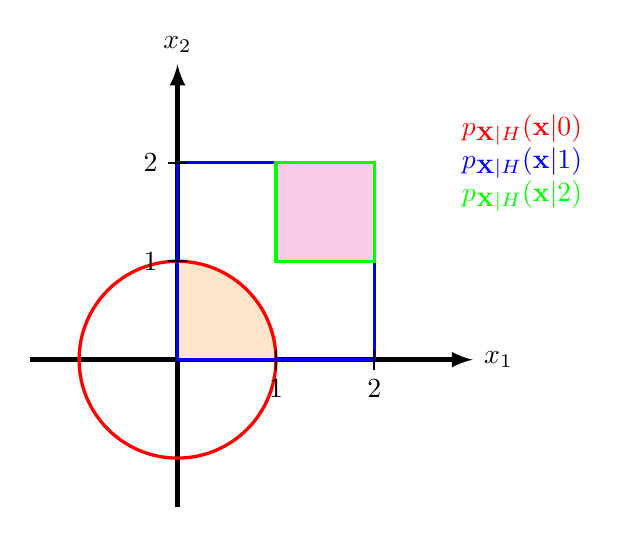
\begin{tikzpicture}[scale=1.25,cap=butt]
  \usetikzlibrary{arrows} % LATEX and plain TEX when using TikZ
  
  % Axis
  \draw[-latex,black,ultra thick] (-1.5,0) -- (3,0) node[right,black] {$x_1$};
  \draw[-latex,black,ultra thick] (0,-1.5) -- (0,3) node[above,black] {$x_2$};
  
  % Supports
  \fill[fill=orange!20] (0,0) -- (1,0) arc[start angle=0, end angle=90, radius=1] -- cycle;
  \fill[fill=magenta!20] (1,1) -- (2,1) -- (2,2) -- (1,2) -- cycle;
  \draw[color=red, very thick](0,0) circle (1);
  \draw[blue, very thick] (0,0) rectangle (2,2);
  \draw[green, very thick] (1,1) rectangle (2,2);
  
  % Ticks
  \draw[black,thick] (2,-0.1) node[below,black] {$2$} -- (2,0.1);
  \draw[black,thick] (1,-0.1) node[below,black] {$1$} -- (1,0.1);
  \draw[black,thick] (-0.1,2) node[left,black] {$2$} -- (0.1,2);
  \draw[black,thick] (-0.1,1) node[left,black] {$1$} -- (0.1,1);
  
    % Legend
  \node[draw,align=left,draw=none] at (3.5,2) {\textcolor{red}{$p_{\mathbf{X}|H}(\mathbf{x}|0)$} \\ \textcolor{blue}{$p_{\mathbf{X}|H}(\mathbf{x}|1)$} \\ \textcolor{green}{$p_{\mathbf{X}|H}(\mathbf{x}|2)$}};
  
\end{tikzpicture}
\end{center}
\ifspanish A partir de esta figura, puede comprobarse que los soportes de las verosimilitudes solamente se solapan en dos regiones, que están sombreadas. Por tanto, solamente necesitamos ver qué producto $p_{X|H}(x|h) P_H(h)$ es mayor en estas regiones. In la región anaranjada, es fácil ver que
\else From this plot, we can see that the supports of the likelihoods only overlap in two regions, which are shaded. Then, we only need to see which $p_{X|H}(x|h) P_H(h)$ is larger in these region. In the orange-shaded area, it is easy to see that
\fi
\begin{equation*}
p_{X|H}(x|0) P_H(0) = \frac{1}{\pi} \cdot \frac{1}{8} < p_{X|H}(x|1) P_H(1) = \frac{1}{4} \cdot \frac{1}{2}, 
\end{equation*}
\ifspanish y, por tanto, en esta región debe decidirse $D=1$. En la región sombreada en magenta, resulta
\else and, therefore, in this region we should decide $D = 1$. In the magenta-shaded area, we have
\fi
\begin{equation*}
p_{X|H}(x|1) P_H(1) = \frac{1}{4} \cdot \frac{1}{2} < p_{X|H}(x|2) P_H(2) = 1 \cdot \frac{3}{8},
\end{equation*}
\ifspanish lo que implica que en esta región debe decidirse $D=2$. Por tanto, las regiones de decisión son
\else which implies that in this region we should decide $D = 2$. Hence, the decision regions are
\fi
\begin{align*}
\mathcal{X}_0 &= \{(x_1, x_2)^T \mid x_1^2 + x_2^2 < 1, x_1 \leq 0\} \cup \{(x_1, x_2)^T \mid x_1^2 + x_2^2 < 1, x_1 > 0, x_2 \leq 0 \}, \\
\mathcal{X}_1 &= \{(x_1, x_2)^T \mid 0 < x_1 \leq 1, 0 < x_2 < 2 \} \cup \{(x_1, x_2)^T \mid 1 < x_1 < 2, 0 < x_2 \leq 1 \}  \\
\mathcal{X}_2 &= \{(x_1, x_2)^T \mid 1 < x_1 < 2, 1 < x_2 < 2 \},
\end{align*}
\ifspanish que se muestan en la figura siguiente \else which are the shaded areas shown in the following figure \fi
  \begin{center}
	        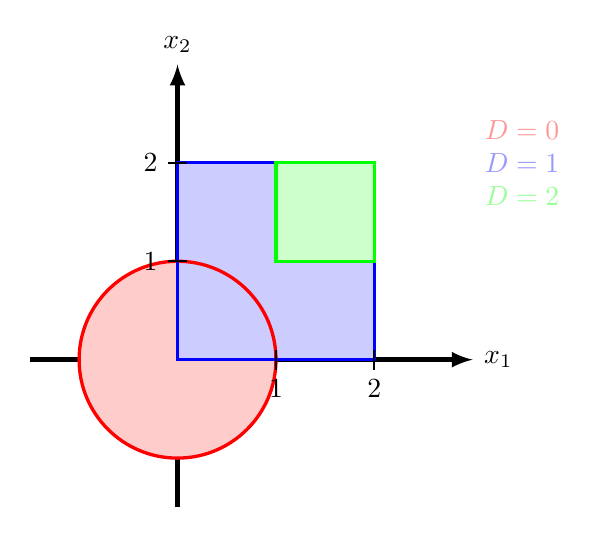
\begin{tikzpicture}[scale=1.25,cap=butt]
  \usetikzlibrary{arrows} % LATEX and plain TEX when using TikZ
  
  % Axis
  \draw[-latex,black,ultra thick] (-1.5,0) -- (3,0) node[right,black] {$x_1$};
  \draw[-latex,black,ultra thick] (0,-1.5) -- (0,3) node[above,black] {$x_2$};
  
  % Supports
  \fill[fill=red!20] (0,0) -- (0,1) arc[start angle=90, end angle=360, radius=1] -- cycle;
  \fill[fill=blue!20] (1,1) -- (2,1) -- (2,0) -- (0,0) -- (0,2) -- (1,2) -- cycle;
  \fill[fill=green!20] (1,1) -- (2,1) -- (2,2) -- (1,2) -- cycle;
  \draw[color=red, very thick](0,0) circle (1);
  \draw[blue, very thick] (0,0) rectangle (2,2);
  \draw[green, very thick] (1,1) rectangle (2,2);
  
  % Ticks
  \draw[black,thick] (2,-0.1) node[below,black] {$2$} -- (2,0.1);
  \draw[black,thick] (1,-0.1) node[below,black] {$1$} -- (1,0.1);
  \draw[black,thick] (-0.1,2) node[left,black] {$2$} -- (0.1,2);
  \draw[black,thick] (-0.1,1) node[left,black] {$1$} -- (0.1,1);
  
  % Legend
  \node[draw,align=left,draw=none] at (3.5,2) {\textcolor{red!40}{$D = 0$} \\ \textcolor{blue!40}{$D = 1$} \\ \textcolor{green!40}{$D = 2$}};
  
\end{tikzpicture}
\end{center}
        
\end{solution}

\part[10]
\ifspanish La probabilidad condicional de la decisión correcta del decisor obtenido, bajo $H = 0$, $P(D = 0 | H = 0)$.
\else The conditional probability of correct decision of the derived detector under $H = 0$, $P(D = 0 | H = 0)$.
\fi
\begin{solution}
\ifspanish La probabilidad pedida es \else The requested probability is \fi
  \begin{equation*}
    P(D = 0 | H = 0) = \int_{\mathcal{X}_0} p_{\mathbf{X}|H}(\mathbf{x}|0) d \mathbf{x}.
  \end{equation*}
\ifspanish Esto, es, se necesita integrar la constante $p_{\mathbf{X}|H}(\mathbf{x}|0) = 1/\pi$ en la region $\mathcal{X}_0$. Sabiendo que $p_{\mathbf{X}|H}(\mathbf{x}|0) = 1/\pi$ integra a $1$ en la región $\{(x_1, x_2)^T \mid x_1^2 + x_2^2 < 1\}$, y se está dejando fuera un cuarto de esa región, resulta
\else That is, we need to integrate the constant $p_{\mathbf{X}|H}(\mathbf{x}|0) = 1/\pi$ in the region $\mathcal{X}_0$. Since we know that $p_{\mathbf{X}|H}(\mathbf{x}|0) = 1/\pi$ integrates to $1$ in the region $\{(x_1, x_2)^T \mid x_1^2 + x_2^2 < 1\}$, and we are leaving out one quarter of that region, $P(D = 0 | H = 0)$ becomes
\fi
\begin{equation*}
P(D = 0 | H = 0) = \frac{3}{4}.
\end{equation*}
  
\end{solution}
  
\end{parts}

